\documentclass[11pt,a4paper]{report}
\usepackage[textwidth=37em,vmargin=30mm]{geometry}
\usepackage{calc,xunicode,amsmath,amssymb,paralist,enumitem,tabu,booktabs,datetime2,xeCJK,xeCJKfntef,listings}
\usepackage{tocloft,fancyhdr,tcolorbox,xcolor,graphicx,eso-pic,xltxtra,xelatexemoji}

\newcommand{\envyear}[0]{2025}
\newcommand{\envdatestr}[0]{2025-05-01}
\newcommand{\envfinaldir}[0]{webdb/2025/20250501/final}

\usepackage[hidelinks]{hyperref}
\hypersetup{
    colorlinks=false,
    pdfpagemode=FullScreen,
    pdftitle={Web Digest - \envdatestr}
}

\setlength{\cftbeforechapskip}{10pt}
\renewcommand{\cftchapfont}{\rmfamily\bfseries\large\raggedright}
\setlength{\cftbeforesecskip}{2pt}
\renewcommand{\cftsecfont}{\sffamily\small\raggedright}

\setdefaultleftmargin{2em}{2em}{1em}{1em}{1em}{1em}

\usepackage{xeCJK,xeCJKfntef}
\xeCJKsetup{PunctStyle=plain,RubberPunctSkip=false,CJKglue=\strut\hskip 0pt plus 0.1em minus 0.05em,CJKecglue=\strut\hskip 0.22em plus 0.2em}
\XeTeXlinebreaklocale "zh"
\XeTeXlinebreakskip = 0pt


\setmainfont{Brygada 1918}
\setromanfont{Brygada 1918}
\setsansfont{IBM Plex Sans}
\setmonofont{JetBrains Mono NL}
\setCJKmainfont{Noto Serif CJK SC}
\setCJKromanfont{Noto Serif CJK SC}
\setCJKsansfont{Noto Sans CJK SC}
\setCJKmonofont{Noto Sans CJK SC}

\setlength{\parindent}{0pt}
\setlength{\parskip}{8pt}
\linespread{1.15}

\lstset{
	basicstyle=\ttfamily\footnotesize,
	numbersep=5pt,
	backgroundcolor=\color{black!5},
	showspaces=false,
	showstringspaces=false,
	showtabs=false,
	tabsize=2,
	captionpos=b,
	breaklines=true,
	breakatwhitespace=true,
	breakautoindent=true,
	linewidth=\textwidth
}






\newcommand{\coverpic}[2]{
    % argv: itemurl, authorname
    Cover photo by #2~~(\href{#1}{#1})
}
\newcommand{\makeheader}[0]{
    \begin{titlepage}
        % \newgeometry{hmargin=15mm,tmargin=21mm,bmargin=12mm}
        \begin{center}
            
            \rmfamily\scshape
            \fontspec{BaskervilleF}
            \fontspec{Old Standard}
            \fontsize{59pt}{70pt}\selectfont
            WEB\hfill DIGEST
            
            \vfill
            % \vskip 30pt
            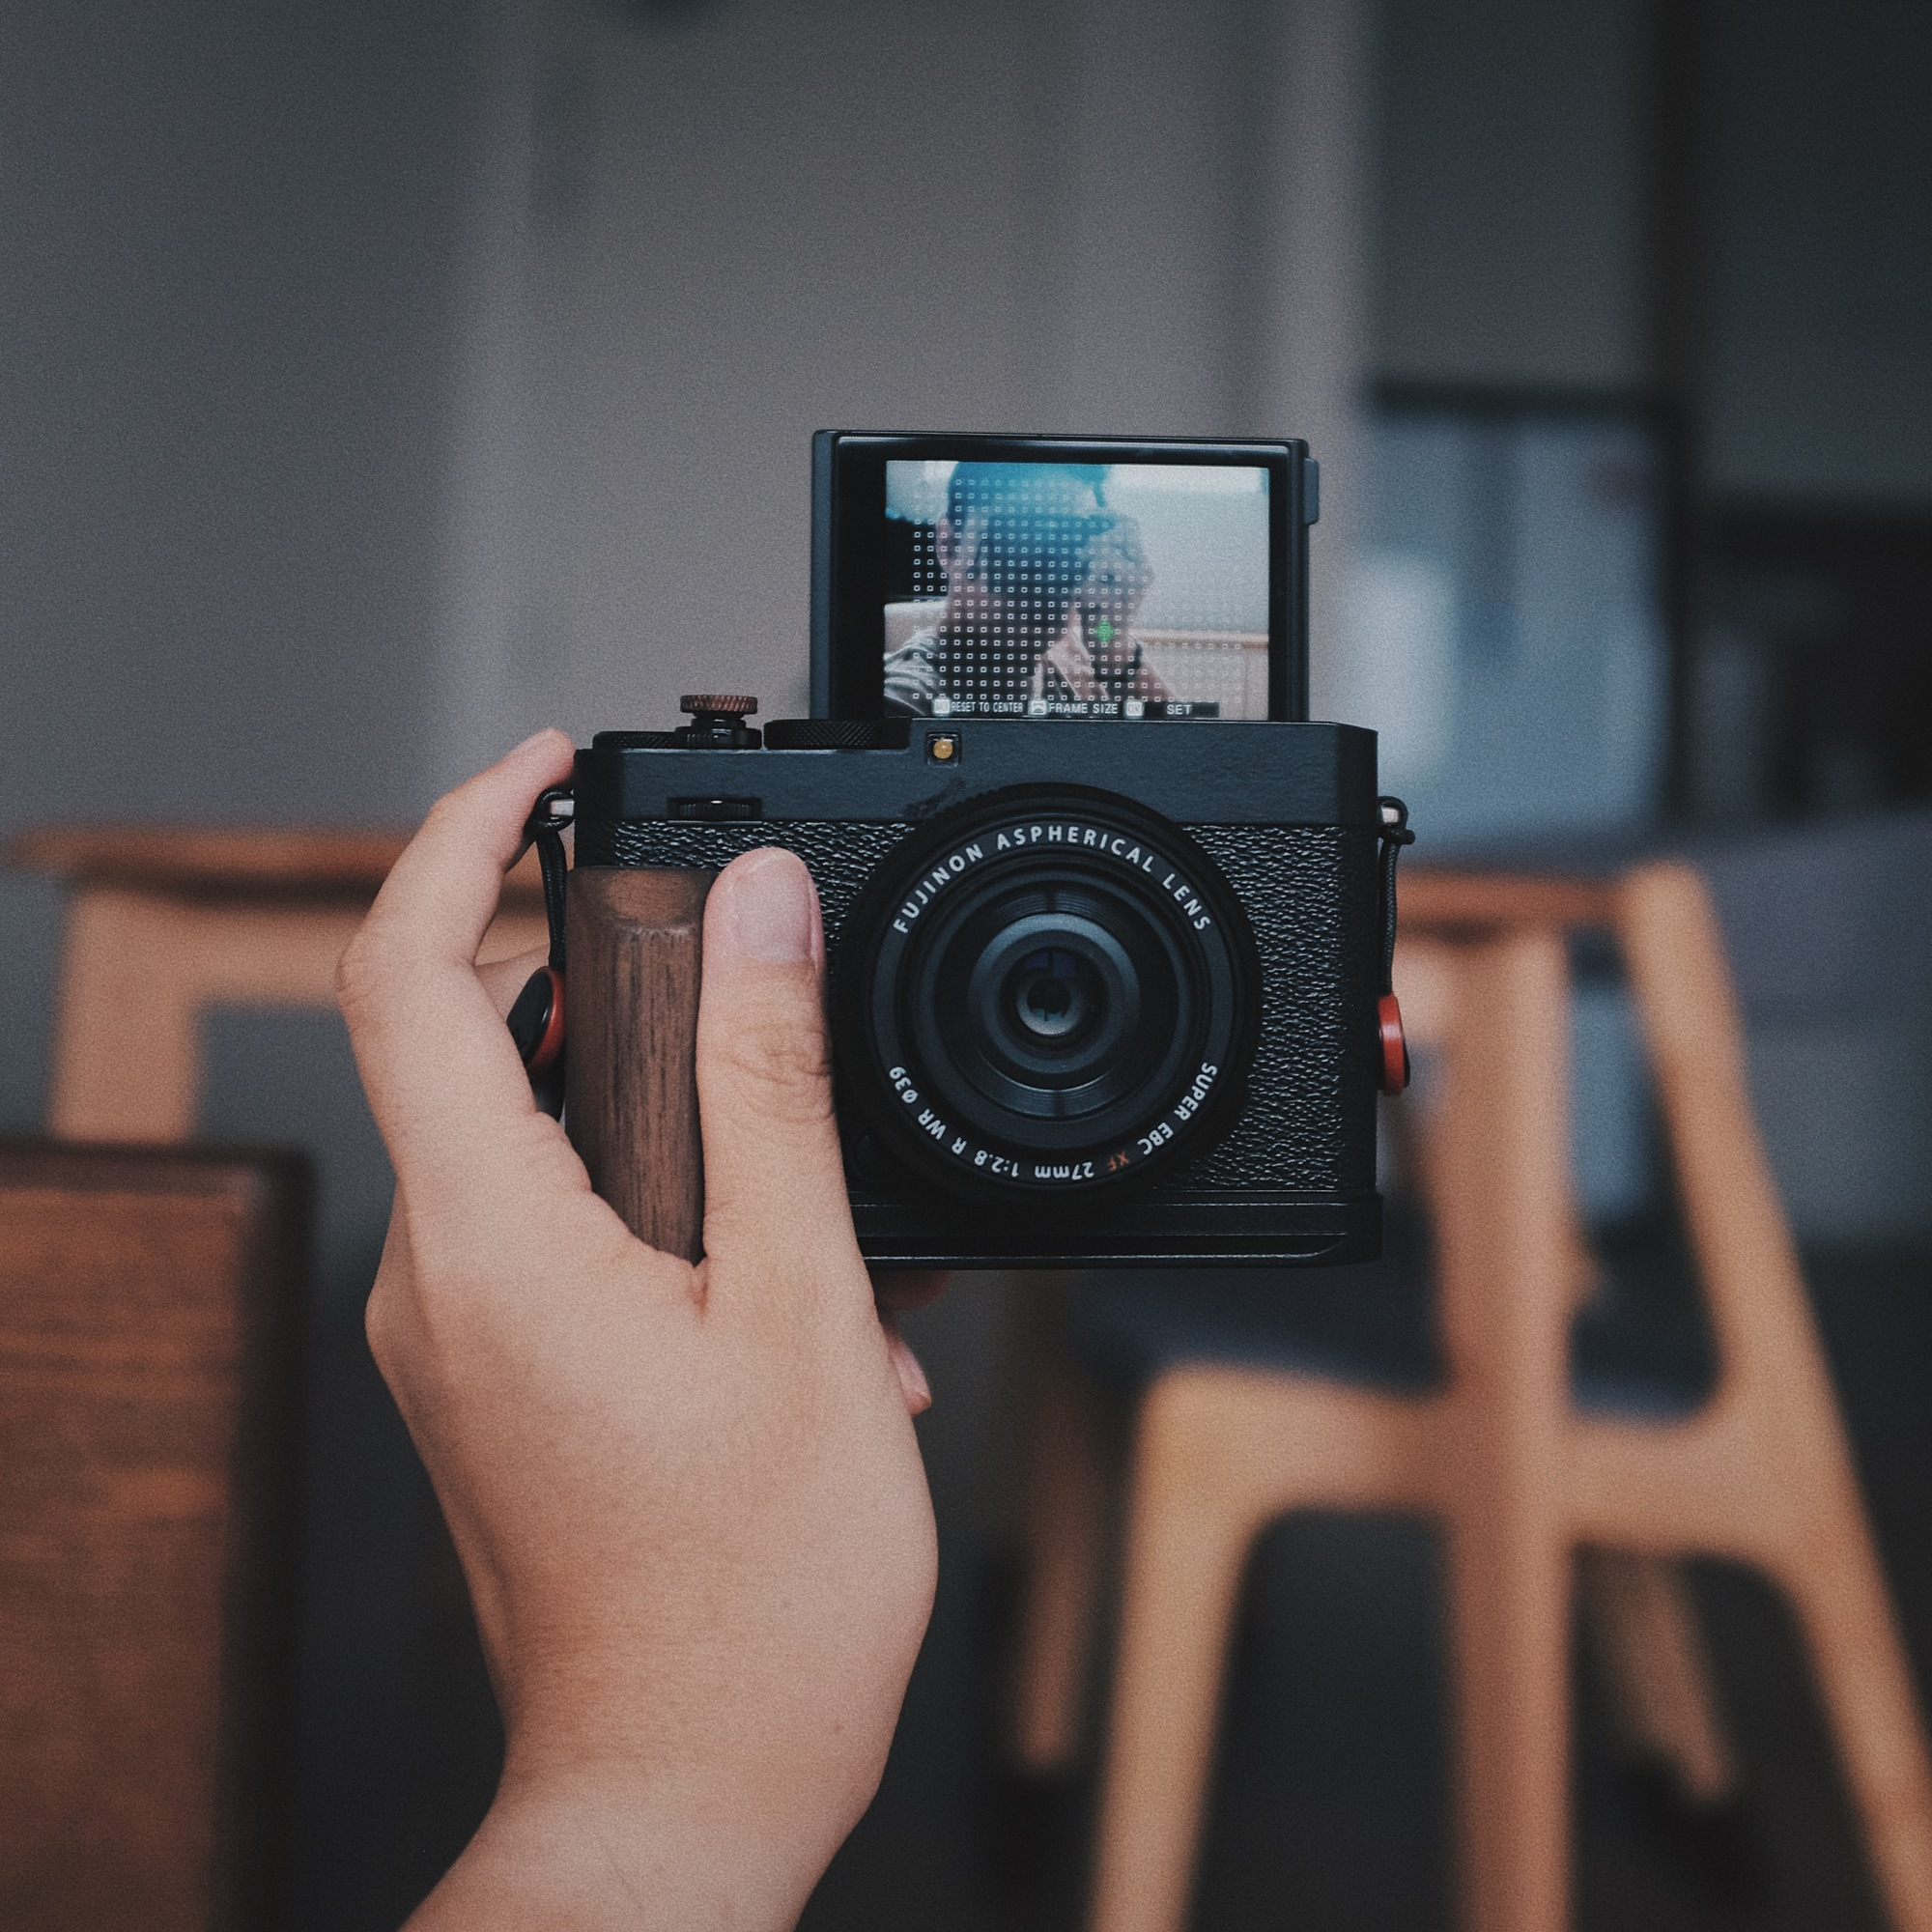
\includegraphics[width=\linewidth]{\envfinaldir/coverpic-prod.jpg}\par
            % \vskip 30pt
            \vfill

            \normalsize\rmfamily\scshape
            \copyright{} The Web Digest Project \hfill\large \envdatestr
        \end{center}
    \end{titlepage}
    % \restoregeometry
}
\newcommand{\simplehref}[1]{%
    \textcolor{blue!80!green}{\href{#1}{#1}}%
}
\renewcommand{\contentsname}{\center\Huge\sffamily\bfseries Contents\par\vskip 20pt}
\newcounter{ipartcounter}
\setcounter{ipartcounter}{0}
\newcommand{\ipart}[1]{
    % \vskip 20pt
    \clearpage
    \stepcounter{ipartcounter}
    \phantomsection
    \addcontentsline{toc}{chapter}{#1}
    % \begin{center}
    %     \Huge
    %     \sffamily\bfseries
    %     #1
    % \end{center}
    % \vskip 20pt plus 7pt
}
\newcounter{ichaptercounter}
\setcounter{ichaptercounter}{0}
\newcommand{\ichapter}[1]{
    % \vskip 20pt
    \clearpage
    \stepcounter{ichaptercounter}
    \phantomsection
    \addcontentsline{toc}{section}{\numberline{\arabic{ichaptercounter}}#1}
    \begin{center}
        \Huge
        \sffamily\bfseries
        #1
    \end{center}
    \vskip 20pt plus 7pt
}
\newcommand{\entrytitlefont}[1]{\subsection*{\raggedright\Large\sffamily\bfseries#1}}
\newcommand{\entryitemGeneric}[2]{
    % argv: title, url
    \parbox{\linewidth}{
        \entrytitlefont{#1}\par\vskip 5pt
        \footnotesize\ttfamily\mdseries
        \simplehref{#2}
    }\vskip 11pt plus 11pt minus 1pt
}
\newcommand{\entryitemGithub}[3]{
    % argv: title, url, desc
    \parbox{\linewidth}{
        \entrytitlefont{#1}\par\vskip 5pt
        \footnotesize\ttfamily\mdseries
        \simplehref{#2}\par\vskip 5pt
        \small\rmfamily\mdseries#3
    }\vskip 11pt plus 11pt minus 1pt
}
\newcommand{\entryitemAp}[3]{
    % argv: title, url, desc
    \parbox{\linewidth}{
        \entrytitlefont{#1}\par\vskip 5pt
        \footnotesize\ttfamily\mdseries
        \simplehref{#2}\par\vskip 5pt
        \small\rmfamily\mdseries#3
    }\vskip 11pt plus 11pt minus 1pt
}
\newcommand{\entryitemHackernews}[3]{
    % argv: title, hnurl, rawurl
    % \parbox{\linewidth}{
    %     \entrytitlefont{#1}\par\vskip 5pt
    %     \footnotesize\ttfamily\mdseries
    %     \simplehref{#3}\par
    %     \textcolor{black!50}{\href{#2}{#2}}
    % }\vskip 11pt plus 11pt minus 1pt
    \begin{minipage}{\linewidth}
            \entrytitlefont{#1}\par\vskip 5pt
            \footnotesize\ttfamily\mdseries
            \simplehref{#3}\par
            \textcolor{black!50}{\href{#2}{#2}}
    \end{minipage}\par\vskip 11pt plus 11pt minus 1pt
}







\begin{document}

\makeheader

\tableofcontents\clearpage




\ipart{Developers}
\ichapter{Hacker News}
\entryitemTwoLinks{Mercury, the first commercial-scale diffusion language model}{https://news.ycombinator.com/item?id=43851099}{https://www.inceptionlabs.ai/introducing-mercury}

\entryitemTwoLinks{JetBrains defends removal of negative reviews for unpopular AI Assistant}{https://news.ycombinator.com/item?id=43850377}{https://devclass.com/2025/04/30/jetbrains-defends-removal-of-negative-reviews-for-unpopular-ai-assistant/}

\entryitemTwoLinks{Google Play sees 47\% decline in apps since start of last year}{https://news.ycombinator.com/item?id=43849383}{https://techcrunch.com/2025/04/29/google-play-sees-47-decline-in-apps-since-start-of-last-year/}

\entryitemTwoLinks{Linux Kernel Exploitation: Attack of the Vsock}{https://news.ycombinator.com/item?id=43849373}{https://hoefler.dev/articles/vsock.html}

\entryitemTwoLinks{Future of OSU Open Source Lab in Jeopardy}{https://news.ycombinator.com/item?id=43849271}{https://osuosl.org/blog/osl-future/}

\entryitemTwoLinks{Reversible computing with mechanical links and pivots}{https://news.ycombinator.com/item?id=43848398}{https://tennysontbardwell.com/blog/2025/04/30/mechanical-computing/index.html}

\entryitemTwoLinks{NotebookLM Audio Overviews are now available in over 50 languages}{https://news.ycombinator.com/item?id=43848325}{https://blog.google/technology/google-labs/notebooklm-audio-overviews-50-languages/}

\entryitemTwoLinks{DeepSeek-Prover-V2}{https://news.ycombinator.com/item?id=43847432}{https://github.com/deepseek-ai/DeepSeek-Prover-V2}

\entryitemTwoLinks{Someone at YouTube needs glasses}{https://news.ycombinator.com/item?id=43846487}{https://jayd.ml/2025/04/30/someone-at-youtube-needs-glasses.html}

\entryitemTwoLinks{Joining Sun Microsystems – 40 years ago (2022)}{https://news.ycombinator.com/item?id=43846187}{https://akapugs.blog/2022/05/03/674/}

\entryitemTwoLinks{"AI-first" is the new Return To Office}{https://news.ycombinator.com/item?id=43845089}{https://www.anildash.com//2025/04/19/ai-first-is-the-new-return-to-office/}

\entryitemTwoLinks{Port of Los Angeles says shipping volume will plummet 35\% next week}{https://news.ycombinator.com/item?id=43844708}{https://www.cnbc.com/2025/04/29/port-of-los-angeles-sees-shipping-volume-down-35percent-next-week-as-tariffs-bite.html}

\entryitemTwoLinks{U.S. Economy Contracts at 0.3\% Rate in First Quarter}{https://news.ycombinator.com/item?id=43844342}{https://www.wsj.com/economy/us-gdp-q1-2025-1f82f689}

\entryitemTwoLinks{Retailers will soon have only about 7 weeks of full inventories left}{https://news.ycombinator.com/item?id=43843821}{https://fortune.com/article/retailers-weeks-of-inventory-left-trump-china-trade-war/}

\entryitemTwoLinks{Secret Deals, Foreign Investments: The Rise of Trump's Crypto Firm}{https://news.ycombinator.com/item?id=43843621}{https://www.nytimes.com/2025/04/29/us/politics/trump-crypto-world-liberty-financial.html}

\entryitemTwoLinks{Finland Bans Smartphones in Schools}{https://news.ycombinator.com/item?id=43842856}{https://yle.fi/a/74-20158886}

\entryitemTwoLinks{Xiaomi MiMo Reasoning Model}{https://news.ycombinator.com/item?id=43842683}{https://github.com/XiaomiMiMo/MiMo}

\entryitemTwoLinks{The Leaderboard Illusion}{https://news.ycombinator.com/item?id=43842380}{https://arxiv.org/abs/2504.20879}

\entryitemTwoLinks{I created Perfect Wiki and reached \$250k in annual revenue without investors}{https://news.ycombinator.com/item?id=43842306}{https://habr.com/en/articles/905812/}

\entryitemTwoLinks{Linux in Excel}{https://news.ycombinator.com/item?id=43840861}{https://github.com/NSG650/LinuxInExcel}\ichapter{Phoronix}
\entryitemGeneric{\hskip 0pt{}Mesa 25.1-rc3 \& Mesa 25.0.5 Deliver More Graphics Driver Fixes}{https://www.phoronix.com/news/Mesa-25.1-rc3-Released}

\entryitemGeneric{\hskip 0pt{}Intel Makes "AI Flame Graphs" Open-Source}{https://www.phoronix.com/news/Intel-AI-Flame-Graphs-Open}

\entryitemGeneric{\hskip 0pt{}Intel's Vulkan Linux Driver Adds Memory Pool Support For Some Massive Performance Gains}{https://www.phoronix.com/news/Intel-Vulkan-Linux-Memory-Pool}

\entryitemGeneric{\hskip 0pt{}openSUSE Leap 16 Available For Beta Testing - Built From SUSE Linux Enterprise 16}{https://www.phoronix.com/news/openSUSE-Leap-16-Beta}

\entryitemGeneric{\hskip 0pt{}LibreSSL 4.1 Released With Faster SHA-1/SHA-256/SHA-512 On Modern AMD \& Intel CPUs}{https://www.phoronix.com/news/LibreSSL-4.1-Released}

\entryitemGeneric{\hskip 0pt{}Bytedance Proposes Faster Linux Inter-Process Communication With "Run Process As Library"}{https://www.phoronix.com/news/Bytedance-Faster-Linux-IPC-RPAL}

\entryitemGeneric{\hskip 0pt{}NVIDIA Posts 60 Patches For Open-Source Hopper \& Blackwell GPU Support On Nouveau}{https://www.phoronix.com/news/NVIDIA-Nouveau-Hopper-Blackwell}

\entryitemGeneric{\hskip 0pt{}Firefox 139 Beta Delivers Faster HTTP/3 Upload Performance}{https://www.phoronix.com/news/Firefox-139-Beta-Released}

\entryitemGeneric{\hskip 0pt{}AMDVLK 2025.Q2.1 Released With More Vulkan Extensions, Hawk Point 1 \& 2 Support}{https://www.phoronix.com/news/AMDVLK-2025.Q2.1-Released}\ichapter{Dribbble}
\entryitemGeneric{\hskip 0pt{}NEW YORK}{https://dribbble.com/shots/25962578-NEW-YORK}

\entryitemGeneric{\hskip 0pt{}Spin Twin // Website}{https://dribbble.com/shots/25960774-Spin-Twin-Website}

\entryitemGeneric{\hskip 0pt{}Aura - Brand System}{https://dribbble.com/shots/25962395-Aura-Brand-System}

\entryitemGeneric{\hskip 0pt{}New Logo Collection}{https://dribbble.com/shots/25960892-New-Logo-Collection}

\entryitemGeneric{\hskip 0pt{}Landing Page DeFi Design}{https://dribbble.com/shots/25961311-Landing-Page-DeFi-Design}

\entryitemGeneric{\hskip 0pt{}Helio}{https://dribbble.com/shots/25955551-Helio}

\entryitemGeneric{\hskip 0pt{}R}{https://dribbble.com/shots/25954740-R}

\entryitemGeneric{\hskip 0pt{}Crypto Exchange Mobile UI}{https://dribbble.com/shots/25955808-Crypto-Exchange-Mobile-UI}

\entryitemGeneric{\hskip 0pt{}Letter F Logos}{https://dribbble.com/shots/25956899-Letter-F-Logos}

\entryitemGeneric{\hskip 0pt{}Sellin UI Kit on UI8 download}{https://dribbble.com/shots/25948738-Sellin-UI-Kit-on-UI8-download}

\entryitemGeneric{\hskip 0pt{}Core 2.0 – Dashboard Builder}{https://dribbble.com/shots/25956157-Core-2-0-Dashboard-Builder}

\entryitemGeneric{\hskip 0pt{}Finergy UIkit on UI8}{https://dribbble.com/shots/25948707-Finergy-UIkit-on-UI8}

\entryitemGeneric{\hskip 0pt{}Clint}{https://dribbble.com/shots/25947599-Clint}

\entryitemGeneric{\hskip 0pt{}Tallybreeze Logo Design - Accounting Automation for Property}{https://dribbble.com/shots/25946704-Tallybreeze-Logo-Design-Accounting-Automation-for-Property}

\entryitemGeneric{\hskip 0pt{}Maybelline // 3D Promo Animation}{https://dribbble.com/shots/25946191-Maybelline-3D-Promo-Animation}

\entryitemGeneric{\hskip 0pt{}Fat Cat Movie Night}{https://dribbble.com/shots/25947610-Fat-Cat-Movie-Night}

\entryitemGeneric{\hskip 0pt{}Progressive RV Insurance Print Ads}{https://dribbble.com/shots/25948535-Progressive-RV-Insurance-Print-Ads}

\entryitemGeneric{\hskip 0pt{}New Personal Website}{https://dribbble.com/shots/25947555-New-Personal-Website}

\entryitemGeneric{\hskip 0pt{}Onboarding screen collection}{https://dribbble.com/shots/25943700-Onboarding-screen-collection}

\entryitemGeneric{\hskip 0pt{}Bismuth}{https://dribbble.com/shots/25942596-Bismuth}

\entryitemGeneric{\hskip 0pt{}Cute Viking Brand Mascot}{https://dribbble.com/shots/25943003-Cute-Viking-Brand-Mascot}

\entryitemGeneric{\hskip 0pt{}Quora Logo Redesign Concept}{https://dribbble.com/shots/25941918-Quora-Logo-Redesign-Concept}

\entryitemGeneric{\hskip 0pt{}Rhino Dragon}{https://dribbble.com/shots/25945050-Rhino-Dragon}

\entryitemGeneric{\hskip 0pt{}Minimalist Z Logo Design // For Sale}{https://dribbble.com/shots/25941466-Minimalist-Z-Logo-Design-For-Sale}


\ipart{Developers~~~~(zh-Hans)}
\ichapter{Solidot}
\entryitemGeneric{\hskip 0pt{}因经济动荡 LWN 考虑涨价}{https://www.solidot.org/story?sid=81193}

\entryitemGeneric{\hskip 0pt{}撞击月球产生的碎片四分之一掉落到地球}{https://www.solidot.org/story?sid=81192}

\entryitemGeneric{\hskip 0pt{}Google 称政府更频繁的使用 0day}{https://www.solidot.org/story?sid=81191}

\entryitemGeneric{\hskip 0pt{}Firefox 138 释出,标签组正式推出}{https://www.solidot.org/story?sid=81190}

\entryitemGeneric{\hskip 0pt{}芬兰议会通过限制中小学生使用手机的法律}{https://www.solidot.org/story?sid=81189}

\entryitemGeneric{\hskip 0pt{}黄金可能来自磁星}{https://www.solidot.org/story?sid=81188}

\entryitemGeneric{\hskip 0pt{}LG 将于 6 月底关闭智能手机更新服务}{https://www.solidot.org/story?sid=81187}

\entryitemGeneric{\hskip 0pt{}Google Play 应用数量减少 47\%}{https://www.solidot.org/story?sid=81186}

\entryitemGeneric{\hskip 0pt{}前苏联失败的金星探测器即将坠落回地面}{https://www.solidot.org/story?sid=81185}

\entryitemGeneric{\hskip 0pt{}入侵餐厅菜单软件修改过敏信息的前迪士尼员工被判三年}{https://www.solidot.org/story?sid=81184}

\entryitemGeneric{\hskip 0pt{}西班牙和葡萄牙大规模停电原因是极端气温变化}{https://www.solidot.org/story?sid=81183}

\entryitemGeneric{\hskip 0pt{}因长时间盯着屏幕年轻一代出现干眼症}{https://www.solidot.org/story?sid=81182}

\entryitemGeneric{\hskip 0pt{}亚马逊将在商品价格中显示关税,白宫谴责}{https://www.solidot.org/story?sid=81181}

\entryitemGeneric{\hskip 0pt{}经济学家发现生成式 AI 没有取代工作或影响薪水}{https://www.solidot.org/story?sid=81180}

\entryitemGeneric{\hskip 0pt{}物质使用通过不同分子途径加速大脑老化}{https://www.solidot.org/story?sid=81179}

\entryitemGeneric{\hskip 0pt{}天然补充剂 Cel System 或有助于延缓衰老}{https://www.solidot.org/story?sid=81178}

\entryitemGeneric{\hskip 0pt{}价值 3.307 亿美元比特币的疑似被盗}{https://www.solidot.org/story?sid=81177}

\entryitemGeneric{\hskip 0pt{}汽车订阅功能增加司机被政府监视风险}{https://www.solidot.org/story?sid=81176}

\entryitemGeneric{\hskip 0pt{}阿里发布新开源权重模型 Qwen3}{https://www.solidot.org/story?sid=81175}

\entryitemGeneric{\hskip 0pt{}亚马逊发射首批互联网卫星}{https://www.solidot.org/story?sid=81174}\ichapter{V2EX}
\entryitemGeneric{\hskip 0pt{}[成都] 成都外包 17k 是个什么水平?}{https://www.v2ex.com/t/1129258}

\entryitemGeneric{\hskip 0pt{}[iPad] iPad 11 (A16) 电源按键松动是通病吗}{https://www.v2ex.com/t/1129256}

\entryitemGeneric{\hskip 0pt{}[分享发现] 苹果这批漏洞,有点严重啊}{https://www.v2ex.com/t/1129255}

\entryitemGeneric{\hskip 0pt{}[问与答] 个人网上冷归档/备份的最佳实践是什么?}{https://www.v2ex.com/t/1129254}

\entryitemGeneric{\hskip 0pt{}[问与答] pollo.ai 免费(有次数)AI 视频工具}{https://www.v2ex.com/t/1129253}

\entryitemGeneric{\hskip 0pt{}[Kubernetes] 再也不用记 k8s 的命令了}{https://www.v2ex.com/t/1129252}

\entryitemGeneric{\hskip 0pt{}[宽带症候群] 关于 "家宽不允许开设 Web 服务" 限制的一些解读}{https://www.v2ex.com/t/1129251}

\entryitemGeneric{\hskip 0pt{}[程序员] 直接用 v0.dev 写的界面与真实的后端接口通讯可以吗?}{https://www.v2ex.com/t/1129249}

\entryitemGeneric{\hskip 0pt{}[问与答] Chrome 光标异常}{https://www.v2ex.com/t/1129248}

\entryitemGeneric{\hskip 0pt{}[优惠信息] 腾讯福袋领取}{https://www.v2ex.com/t/1129247}

\entryitemGeneric{\hskip 0pt{}[问与答] 预算 2000 该买洋垃圾还是 nas}{https://www.v2ex.com/t/1129246}

\entryitemGeneric{\hskip 0pt{}[推广] 程序员做了 4 个月百家号,百度还真给我打钱了,不多就 500 元!}{https://www.v2ex.com/t/1129244}

\entryitemGeneric{\hskip 0pt{}[问与答] 求推荐 8k-10k 办公笔记本电脑}{https://www.v2ex.com/t/1129243}

\entryitemGeneric{\hskip 0pt{}[Terminal] 开发和运维喜欢的终端客户端的区别}{https://www.v2ex.com/t/1129242}

\entryitemGeneric{\hskip 0pt{}[宽带症候群] 给版友们分享点你们肯定感兴趣的细糠(Cisco Dell Fortinet 等原厂授权的 1/12 微缩网络设备模型及机架)}{https://www.v2ex.com/t/1129240}

\entryitemGeneric{\hskip 0pt{}[生活] 国内的电商为什么这么喜欢同步的交流方式}{https://www.v2ex.com/t/1129239}

\entryitemGeneric{\hskip 0pt{}[iPhone] iPhone 自带中文输入法 语音按钮时不时灰色}{https://www.v2ex.com/t/1129238}

\entryitemGeneric{\hskip 0pt{}[分享创造] 一个 side project httpspot.dev httpbin 的替代}{https://www.v2ex.com/t/1129237}

\entryitemGeneric{\hskip 0pt{}[求职] 求解,学历升级相关方面}{https://www.v2ex.com/t/1129236}

\entryitemGeneric{\hskip 0pt{}[优惠信息] 分享几个自用 JiChang 的五一优惠码}{https://www.v2ex.com/t/1129235}

\entryitemGeneric{\hskip 0pt{}[DevOps] tg 上运维/sre/devops 相关的交流群}{https://www.v2ex.com/t/1129234}

\entryitemGeneric{\hskip 0pt{}[吉他] 新手入门吉他,不仅要会弹,还要会唱吗}{https://www.v2ex.com/t/1129233}

\entryitemGeneric{\hskip 0pt{}[宽带症候群] 上海联通宽带测速不正常}{https://www.v2ex.com/t/1129231}

\entryitemGeneric{\hskip 0pt{}[程序员] 求问 2025 年技术栈选择, RN 还是 flutter}{https://www.v2ex.com/t/1129229}

\entryitemGeneric{\hskip 0pt{}[macOS] macos 如何查看 GPU 占用率}{https://www.v2ex.com/t/1129228}

\entryitemGeneric{\hskip 0pt{}[问与答] vercel 的 v0.dev 怎么继续编辑一个已存在的项目?}{https://www.v2ex.com/t/1129227}

\entryitemGeneric{\hskip 0pt{}[问与答] 我靠,今天被喷出翔了}{https://www.v2ex.com/t/1129226}

\entryitemGeneric{\hskip 0pt{}[微软] 微软 Authenticator 变更:将在 25 年 7 月停用自动填充功能, 8 月「已保存的密码」不能再访问}{https://www.v2ex.com/t/1129225}

\entryitemGeneric{\hskip 0pt{}[生活] 老哥们,你们也会背痛吗?}{https://www.v2ex.com/t/1129224}

\entryitemGeneric{\hskip 0pt{}[VPS] 有人在 zgocloud?,最近是不是有点抽风?}{https://www.v2ex.com/t/1129221}

\entryitemGeneric{\hskip 0pt{}[MacBook Pro] M1 Pro 16 寸 虚拟机 玩 GTA V 能开最高分辨率 60hz? 有大佬试过吗?}{https://www.v2ex.com/t/1129220}

\entryitemGeneric{\hskip 0pt{}[宽带症候群] 突然发现国内支持 tcp 的 dns 也不多啊}{https://www.v2ex.com/t/1129219}

\entryitemGeneric{\hskip 0pt{}[分享创造] [开源公测] [安卓端最强直连工具] Cealer (Sheas Cealer 安卓端) [开源 SNI 伪造工具]}{https://www.v2ex.com/t/1129218}

\entryitemGeneric{\hskip 0pt{}[问与答] 如何保持热爱学习的心态?}{https://www.v2ex.com/t/1129216}

\entryitemGeneric{\hskip 0pt{}[Go 编程语言] [Golang/k8s] 内存分析中 pprof 与 runtime 包的 HeapInuse 的 GAP 在哪里呢?}{https://www.v2ex.com/t/1129215}

\entryitemGeneric{\hskip 0pt{}[软件] 目前有什么简单、好用的 pdf 去水印工具?}{https://www.v2ex.com/t/1129214}

\entryitemGeneric{\hskip 0pt{}[分享发现] 五一路途无聊,大家来分享下电影 or 游戏}{https://www.v2ex.com/t/1129213}

\entryitemGeneric{\hskip 0pt{}[问与答] github 上的扩展安装}{https://www.v2ex.com/t/1129212}

\entryitemGeneric{\hskip 0pt{}[RSS] Hacker News 中文 RSS 订阅}{https://www.v2ex.com/t/1129211}

\entryitemGeneric{\hskip 0pt{}[分享发现] 这款 AI 翻译软件可以替换系统翻译 APP 了!}{https://www.v2ex.com/t/1129210}

\entryitemGeneric{\hskip 0pt{}[反馈] 发现了一个 bug,回帖偶发会扣除 5.02 铜币}{https://www.v2ex.com/t/1129209}

\entryitemGeneric{\hskip 0pt{}[macOS] 送几个音乐播放器的兑换码}{https://www.v2ex.com/t/1129208}

\entryitemGeneric{\hskip 0pt{}[程序员] 哪一家 AI 对会话隐私保护的最好?}{https://www.v2ex.com/t/1129207}

\entryitemGeneric{\hskip 0pt{}[Apple] raycast 出 ios 版了}{https://www.v2ex.com/t/1129206}

\entryitemGeneric{\hskip 0pt{}[程序员] 月兔编程语言支持国产芯片开发,对标 C?}{https://www.v2ex.com/t/1129205}

\entryitemGeneric{\hskip 0pt{}[问与答] 有没有好心人,推荐一个宝藏育儿嫂的?}{https://www.v2ex.com/t/1129203}

\entryitemGeneric{\hskip 0pt{}[程序员] Deepseek 发布新模型}{https://www.v2ex.com/t/1129202}

\entryitemGeneric{\hskip 0pt{}[问与答] api 网关负责 http --> GRPC 的转换吗?}{https://www.v2ex.com/t/1129200}

\entryitemGeneric{\hskip 0pt{}[分享创造] [产品自荐] 基于 Excalidraw 做了一个 AI 生成流程图的试验性工具(手绘风格)}{https://www.v2ex.com/t/1129199}

\entryitemGeneric{\hskip 0pt{}[程序员] Cursor 帮我写了个 pdf 编辑器}{https://www.v2ex.com/t/1129198}


\ipart{Generic News}
\ichapter{联合早报}
\entryitemWithDescription{黎康:魔都的B面}{https://www.zaobao.com/news/china/story20250426-6241474}{``确实这几年上海的城市公共建设很好,但你有没有去看过一些老旧小区的环境?小区里电线横飞,绿化基本毫无规划;进入楼道,你会感觉回到20年前\ldots\ldots'' 上一篇``早点------沪上闲语''发表后,收到一封读者来信。这位上海市民告诉我,在装点城市门面的郁金香背后,如果走进上海的老旧小区,会看到这座城市的另一面……}

\entryitemWithDescription{新闻人间:从``不懂球的胖子''到改革推手——刘国梁}{https://www.zaobao.com/news/china/story20250426-6238850}{中国乒乓球协会星期三(4月23日)突然宣布,刘国梁主动辞去主席一职。这一消息迅速引发体坛热议,有球迷为他的离开感到惋惜,也有体育评论员开始审视他在任期内的功与过。 刘国梁自2018年起担任乒协主席,如今在第二任期尚未结束之际中途请辞,外界难免有诸多猜测。星期三当天,他以主席身份在乒协会议上作最后一次发言时,几度哽咽,甚至当场落泪。 他在记者会上透露,早在去年巴黎奥运会结束后,便已向上级表达了去意……}

\entryitemWithDescription{中国据报考虑暂停加征部分美国产品125\%关税}{https://www.zaobao.com/news/china/story20250425-6245926}{中国政府据报考虑暂停对部分美国进口产品加征125\%的关税,受访学者认为此举主要考虑中国企业的生存需要,与中美是否开启贸易谈判无关。 据彭博社引述知情人士报道,中国政府正考虑取消对美国的医疗设备,以及乙烷等工业化学品加征的报复性关税。中国是全球最大的塑料制造国,但部分工厂依赖从美国进口的乙烷。中国医院也需要美国生产的磁共振成像和超声仪器等医疗设备。 知情人士称,飞机租赁也可能豁免关税……}

\entryitemWithDescription{中国美国商会白皮书:五分之一美企不再视中国为优先投资地}{https://www.zaobao.com/news/china/story20250425-6245113}{中国美国商会的调查显示,五分之一的在华美国企业不再将中国列为优先的投资目的地。 该商会星期五(4月25日)发布由100余名中国美国商会会员企业代表共同撰写的2025年《美国企业在中国白皮书》。 白皮书指出,中美两国关系日益紧张,已连续五年成为在华美资企业面临的首要商业挑战,超过了合规风险和来自中国企业的竞争压力……}

\entryitemWithDescription{中国发布生态调查报告 称菲律宾捕捞现场发现人为弃置物}{https://www.zaobao.com/news/china/story20250425-6244616}{(北京讯)中国多家自然生态机构星期五(4月25日)联合公布一份调查报告,评估铁线礁、牛轭礁珊瑚礁的生态系统状况,称菲律宾所谓``中国在铁线礁倾倒珊瑚碎屑等言论''毫无科学和事实依据。 中国自然资源部微信公号分别发表了这份题为《铁线礁、牛轭礁珊瑚礁生态系统调查报告》的中英文版本,参与编制的机构包括中国自然资源部南海发展研究院、南海生态中心等……}

\entryitemWithDescription{香港公共场所明年起设更多禁烟区 违例罚款提高一倍}{https://www.zaobao.com/news/china/story20250425-6245064}{为了进一步降低吸烟率,香港特区政府将由明年起在更多公共场所设立禁烟区,并把违例吸烟的罚款金额提高一倍至3000港元(508新元)。 相关条例草案星期五(4月25日)刊宪,列明从明年元旦起,禁止在等候公共交通工具、等候进入电影院、医院、公众游乐场地、体育场等地方的划定范围吸烟。违者罚款由1500港元倍增至3000港元……}

\entryitemWithDescription{两韩国顶尖半导体专家 退休后被中国高校任用}{https://www.zaobao.com/news/china/story20250425-6244895}{(首尔讯)中国正通过从海外引进顶尖人才,与美国争夺高科技主导权。韩国两名``国宝级''顶尖专家退休后在本国受到冷落,未能找到合适研究职位,目前已被中国高等学府任用。 据韩国《中央日报》报道,韩国知名碳纳米管专家李永熙去年11月正式受聘于湖北工业大学半导体与量子研究所……}

\entryitemWithDescription{美国传降对陆关税又强化对台论述 分析:谈判或拿台湾当筹码}{https://www.zaobao.com/news/china/story20250425-6244227}{华盛顿释出降低对华关税信号、寻求谈判之际,美国星期三(4月23日)首次在联合国安理会批评北京误用联大2758号决议;更在同一天派遣军舰穿越台湾海峡。受访学者分析,这些作为现阶段暂与关税战没有直接关联,但不排除美国总统特朗普接下来可能利用台湾问题作为对华谈判筹码。 特朗普本周透露考虑大幅度降低对华关税,希望与中国达成``公平的协议'',同时又声称美国每天都同中国直接联系……}

\entryitemWithDescription{韩咏红:特朗普关税从``解放日''走到``妥协日''了?}{https://www.zaobao.com/news/china/story20250425-6240846}{美国总统特朗普在4月2日宣布对等关税政策,短短20天后,特朗普的高姿态已难以为继。特朗普在4月9日就已调整过一次战术,暂缓对其他国家课征对等关税,集中火力单挑中国;而今,特朗普恐怕又要眨眼了,对中国商品课征的145\%关税也可能显著下调。 特朗普近日罕见地对中国伸出橄榄枝,表示考虑大幅度降低对华关税,显露出急于与中国达成协议。但中国偏是表现得不着急……}

\entryitemWithDescription{学者:中国以2+2机制拉拢东南亚国家抗衡美国}{https://www.zaobao.com/news/china/story20250424-6240690}{受访学者分析,在中美关系因贸易战而全面恶化的大背景下,中国正以``外交、国防2+2对话机制''为新抓手,积极拉拢亚细安成员国,以抗衡美国在本区域的影响力,预计中国接下来将推动与更多区域国家建立2+2机制。 中国和印度尼西亚星期一(4月21日)在北京举行外长、防长对话机制下的首次部长级会议,两国在2023年就建立2+2对话机制。中国官方称,这是中国在全球建立的首个部长级2+2机制……}

\entryitemWithDescription{中埃空军首次联训 学者:中国初步具备向中东快速战略投送能力}{https://www.zaobao.com/news/china/story20250424-6240357}{中国空军上周派出多架战斗机、预警机、运输机与空中加油机前往埃及,进行两军首次联训。这是中国空军首次以完整作战体系进行跨洲机动。 受访学者认为,这是中国空军现代化进程的里程碑,有助于发展长途奔袭的技战术;这也标志着中国初步具备向中东进行快速战略投送的能力。 据中国国防部消息,中国与埃及两国空军于4月中旬至5月上旬,在埃及空军基地组织代号为``文明之鹰-2025''的联合训练……}

\entryitemWithDescription{台湾收紧民众申领大陆证照规定 持大陆定居证也将被撤销台湾身份}{https://www.zaobao.com/news/china/story20250424-6239789}{(台北综合讯)台湾再度收紧民众申领中国大陆证照的规定,持有大陆定居证的台湾民众也触犯相关法令,将丧失台湾身份。 综合《旺报》与《联合报》报道,台湾行政院公报显示,陆委会近日对《两岸条例》当中规定发布解释函令称,为确保两岸人员单一身份制度,两岸条例规定台湾人民不得在大陆地区``设有户籍'',或领用大陆地区护照,否则将丧失台湾身份……}

\entryitemWithDescription{神舟二十号成功发射 航天员将开展中国首次涡虫空间再生实验}{https://www.zaobao.com/news/china/story20250424-6239950}{(北京综合讯)中国星期四(4月24日)成功发射神舟二十号载人飞船。三名航天员将在空间站驻留约六个月,并开展中国首次涡虫空间再生实验。 综合新华社、央视新闻和《中国青年报》报道,搭载神舟二十号的长征二号F遥二十运载火箭,星期四下午5时17分在甘肃酒泉卫星发射中心点火发射。约10分钟后,神舟二十号与火箭成功分离,进入预定轨道……}

\entryitemWithDescription{台大罢免升温 朝野对抗加剧}{https://www.zaobao.com/news/china/story20250424-6240062}{台湾两大在野党将携手举办大型造势活动,抗议政府利用司法整肃异己,进行大罢免。兼任民进党主席的总统赖清德则公开肯定公民团体罢免在野党立委的行动影片,检调也持续搜索在野国民党宜兰县党部,朝野对抗情势正逐步升温……}

\entryitemWithDescription{美国国会罕见动用传唤权 调查中国三电信巨头}{https://www.zaobao.com/news/china/story20250424-6239456}{(纽约路透电)美国众议院中国问题特别委员会星期三(4月23日)罕见地动用传唤权,调查中国三大电信公司涉嫌支持中国军方和政府的行为。 据路透社报道,中国移动、中国电信和中国联通三家中国电信巨头收到该委员会的传唤通知,须回答他们是否可通过在美开展的云服务和互联网业务获取美国数据的问题。 美国两党议员持续对被指由中国主导的网络攻击事件表示担忧……}

\entryitemWithDescription{浙江一小学门外发生汽车冲撞人群事件}{https://www.zaobao.com/news/china/story20250424-6238514}{(香港综合讯)中国再发生校园伤人事件,浙江金华一所小学门外星期二(4月22日)放学时有汽车冲撞人群,伤亡人数不明。官方在事发两日后仍未发布通报,中国社媒上的相关信息均被删除。 综合《明报》《南华早报》和网媒``香港01''报道,这起事件发生在金华市苏孟乡中心小学门口,时间是星期二傍晚5时45分左右,正值放学时间。附近商户披露,有多名学生被撞……}

\entryitemWithDescription{学者:关税战伤敌一千自损八百 中美终将找到共处之道}{https://www.zaobao.com/news/china/story20250424-6238821}{美国总统特朗普祭出对等关税将届满一个月,如今传出可能降低对华关税,定居美国的资深华人学者赵全胜指出,中美领导阶层有一批人长期相信对方马上要垮台,但关税战让双方意识到,这无疑是``伤敌一千,自损八百'',因此迟早会找到共处之道。 特朗普4月2日宣布全面实施对等关税,随后在9日紧急暂缓90天,让各国争取与美国谈判的时间与空间,唯独对中国不断加码;北京也不甘示弱,提出相应反制……}

\entryitemWithDescription{打击电诈犯罪扩至纵深地带 缅甸向中国移交920余名嫌犯}{https://www.zaobao.com/news/china/story20250424-6238307}{(北京综合讯)中国与缅甸加大打击电信网络诈骗犯罪合作力度,两国最近一个月的合作执法行动,已从缅北地区扩大到当阳、勐休等缅甸纵深地带。 中国公安部官网星期三(4月23日)通报,缅甸执法部门近日将在当地抓获的920余名中国籍涉诈犯罪嫌疑人,通过云南西双版纳打洛口岸全部移交中国警方。 通报称,缅北电诈犯罪集团遭受重创,但部分涉诈人员为逃避打击,向当阳、勐休等纵深地带转移藏匿,继续实施跨境电诈……}

\entryitemWithDescription{沈泽玮:魔幻山城的中国式现代化演绎}{https://www.zaobao.com/news/china/story20250424-6234868}{时隔12年因工作再访重庆,春夏交替之际迎来烈日当空,与当年冬季旅游行走于山城迷雾的印象截然不同。 5000架无人机灯光秀,既展现科技力量也打造视觉盛宴;科企创始人讲述营商环境不断优化;村委会主任手捧涪陵榨菜分享东方酱腌菜``走出去''成果;火车司机传递通关速度如何带动互联互通跨境贸易;公安局交巡警总队科研处综合科科长讲述数字化赋能超大城市治理;社区党委书记分享中国特色``民主村''的前身今世……}

\entryitemWithDescription{中国网购平台将全面取消``仅退款''}{https://www.zaobao.com/news/china/story20250423-6234242}{在中国官方整治``内卷式竞争''的背景下,中国电商平台将全面取消``仅退款''选项。受访学者认为,此举有助行业回归良性竞争,是对电商市场的一次纠偏。 据《北京商报》报道,拼多多、淘宝、抖音、快手、京东等多个中国电商平台,星期二(4月22日)修改有关``仅退款''的相关条款,消费者申请``退款不退货'',将由商家自主处理……}

\entryitemWithDescription{3月人民币跨境收付占比刷新历史纪录}{https://www.zaobao.com/news/china/story20250423-6233857}{(华盛顿彭博电)随着美元的全球吸引力减弱、中美贸易紧张局势上升,3月中国投资者和贸易公司在国际结算中对人民币的使用大幅增加,创下历史纪录。 彭博社基于中国国家外汇管理局星期二(4月22日)公布的数据计算,3月中国大陆境内个人和机构的跨境业务中,人民币使用占比达 54.3\%,总额7249亿美元(9502亿新元)……}






\clearpage
\leavevmode\vfill
\footnotesize

Copyright \copyright{} 2023-2025 Neruthes and other contributors.

This document is published with CC BY-NC-ND 4.0 license.

The entries listed in this newsletter may be copyrighted by their respective creators.

This newsletter is generated by the Web Digest project.

The newsletters are also delivered via Telegram channel \CJKunderline{\href{https://t.me/webdigestchannel}{https://t.me/webdigestchannel}}.\\
RSS feed is available at \CJKunderline{\href{https://webdigest.pages.dev/rss.xml}{https://webdigest.pages.dev/rss.xml}}.

This newsletter is available in PDF at
\CJKunderline{\href{https://webdigest.pages.dev/}{https://webdigest.pages.dev/}}.

The source code being used to generate this newsletter is available at\\
\CJKunderline{\href{https://github.com/neruthes/webdigest}{https://github.com/neruthes/webdigest}}.

This newsletter is also available in
\CJKunderline{\href{http://webdigest.pages.dev/readhtml/\envyear/WebDigest-20250501.html}{HTML}} and
\CJKunderline{\href{https://github.com/neruthes/webdigest/blob/master/markdown/\envyear/WebDigest-20250501.md}{Markdown}}.


\coverpic{https://unsplash.com/photos/mountains-and-a-lake-under-a-cloudy-sky-4dfNWybkf10}{Cat Guffin}


\end{document}
